\documentclass{article}
% option ``report'' puts title on separate page

\usepackage{amsmath}
\usepackage[pdftex]{graphicx}

\begin{document}

\title{WS6: Advection Equation}
\author{Jackie Villadsen}
\date{\today}
\maketitle


The advection equation operates on spatial function $f(x)$, causing it to translate by ${\Delta}x=vt$ at time
t.  I applied the advection equation with v=0.1 to a Gaussian.

\section{Upwind and Downwind Methods}
\begin{figure}[h]
  \begin{center}
     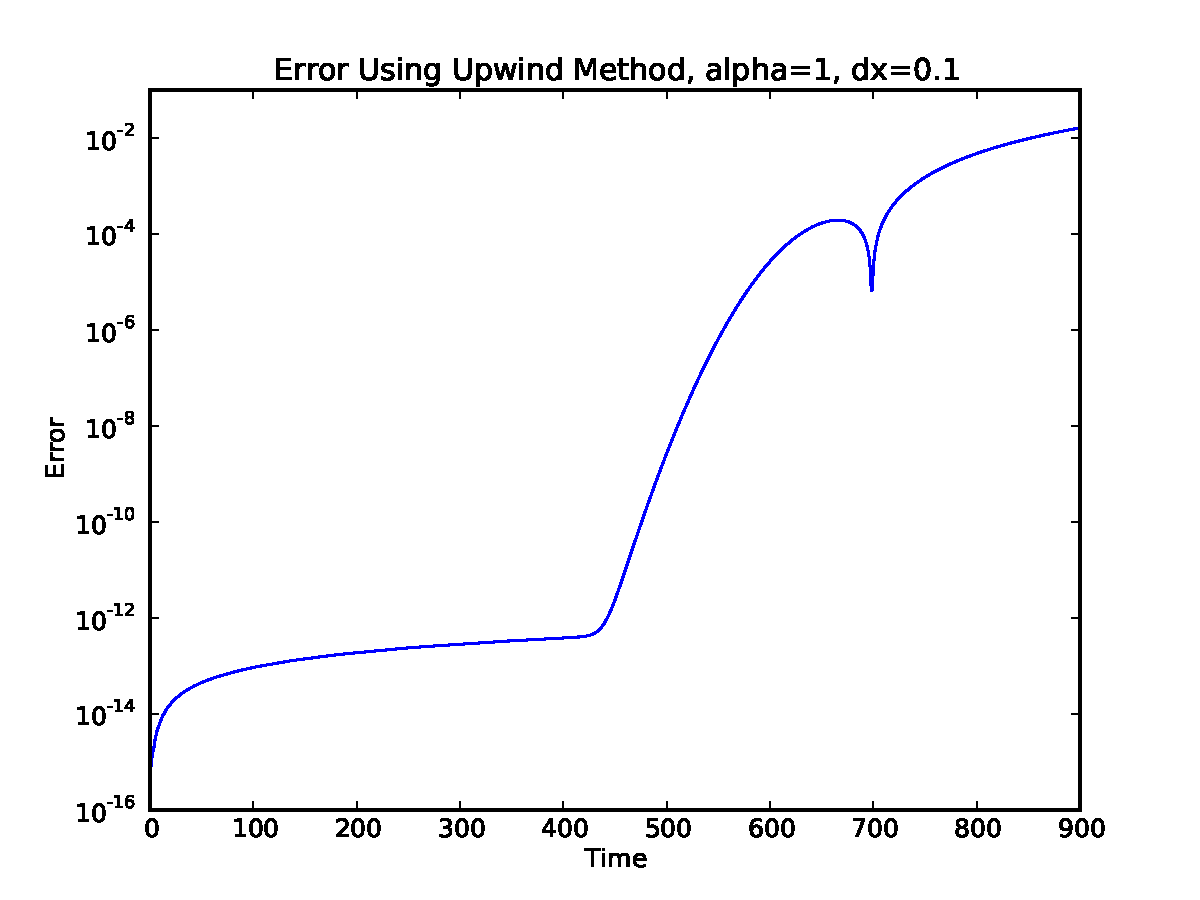
\includegraphics[width=\textwidth]{errfwd}
  \end{center}
  \label{fig:errfwd}
\end{figure}

\begin{figure}[h]
  \begin{center}
     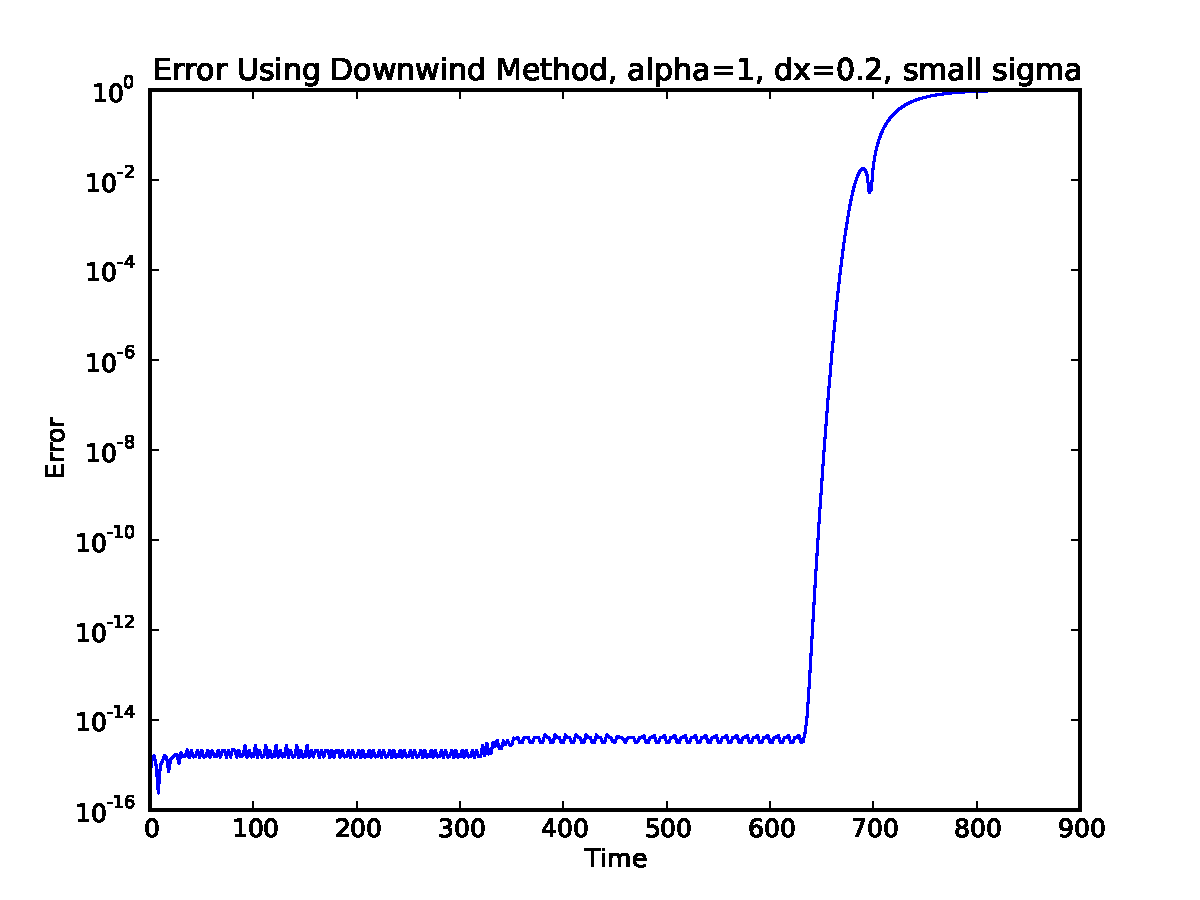
\includegraphics[width=\textwidth]{errfwd_smallsig}
  \end{center}
  \label{fig:errfwd_smallsig}
\end{figure}

Since v is positive, the upwind method is conditionally stable and the downwind method is
unstable.  The upwind method is stable for $\alpha$ between 0 and 1.  With $\alpha=1$, the upwind method
preserved a very small error until the Gaussian slid out of the window (at which point the fractional error
became large because it essentially involved dividing by zero).  I tried $\alpha$ of 0.1 and 0.5.  Both maintained
a Gaussian shape, but it shrank and grew wider over time.  This was much better than for negative $\alpha$ and
$\alpha$ greater than 1.  In both of these cases, as with the downwind method for all $\alpha>0$, the function
would suddenly start to oscillate, and as time progressed more and more oscillations appeared.  The downwind method
was ``stable'' for $\alpha$ from 0 to -1, because then it's just time-reversed upwind for $-\alpha$.

I re-ran my code with the standard deviation of the Gaussian reduced by a factor of 5.  I also reduced the step
size $dx$ by a factor of 5 so that the Gaussian would still be adequately sampled.  Figures \ref{fig:errfwd}
and \ref{fig:errfwd_smallsig} compare the error over time for $\sigma=\sqrt{15}$ and $\sigma=\sqrt{15}/5$, respectively.
For the smaller $\sigma$, the fractional error remained small for longer, but then when it grew, it grew quickly to
a larger value.

\section{FTCS}
For the advection equation, FTCS is unconditionally unstable.  Figures \ref{fig:ftcs5} through \ref{fig:ftcs20}
show the onset of instability over time with the FTCS method, using $\alpha=0.5$ and $dx=1$.  The instability develops
because the positive slope on the left side of the Gaussian results in FTCS predicting negative values incorrectly.

\begin{figure}[h]
  \begin{center}
     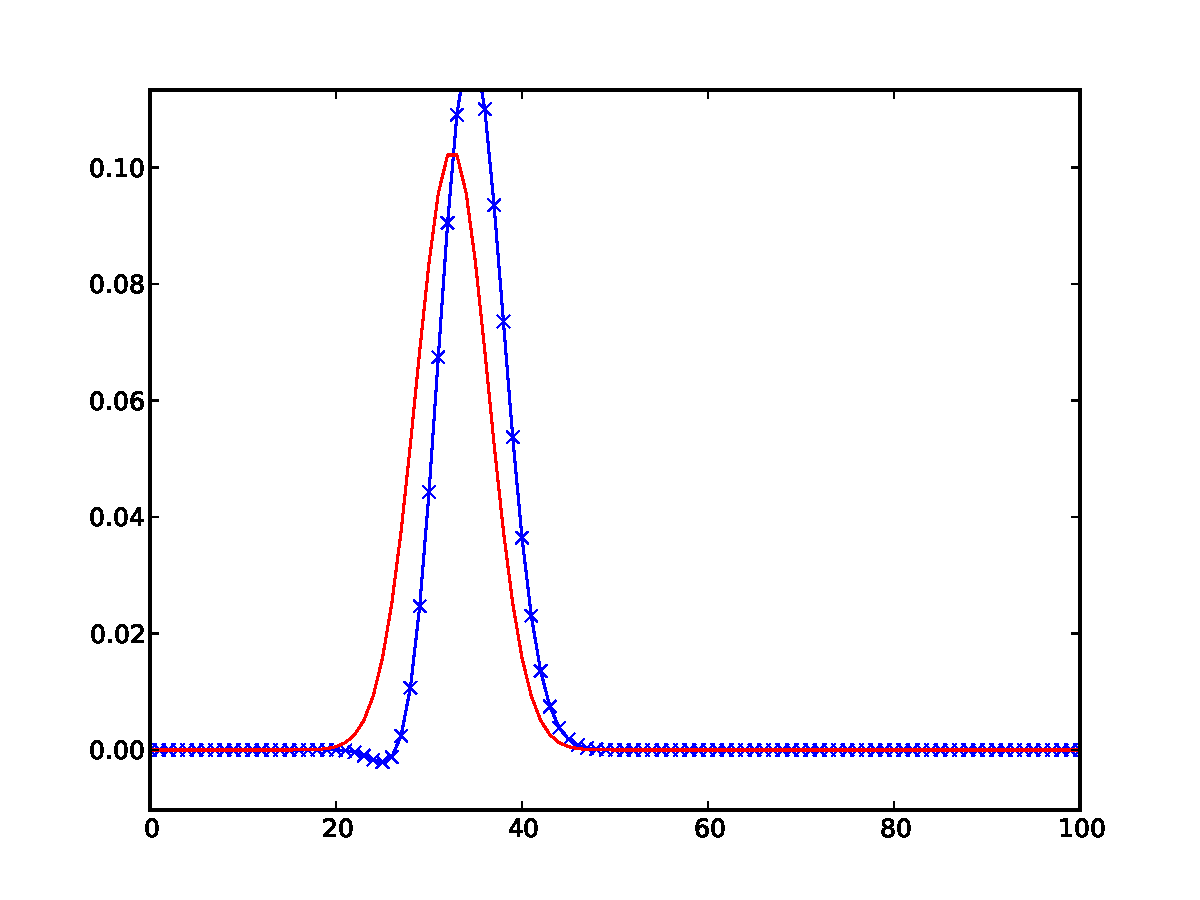
\includegraphics[width=0.5\textwidth]{ftcs5}
  \end{center}
  \label{fig:ftcs5}
  \caption{The evolution of the Gaussian using FTCS after 5 time steps.}
\end{figure}

\begin{figure}[h]
  \begin{center}
     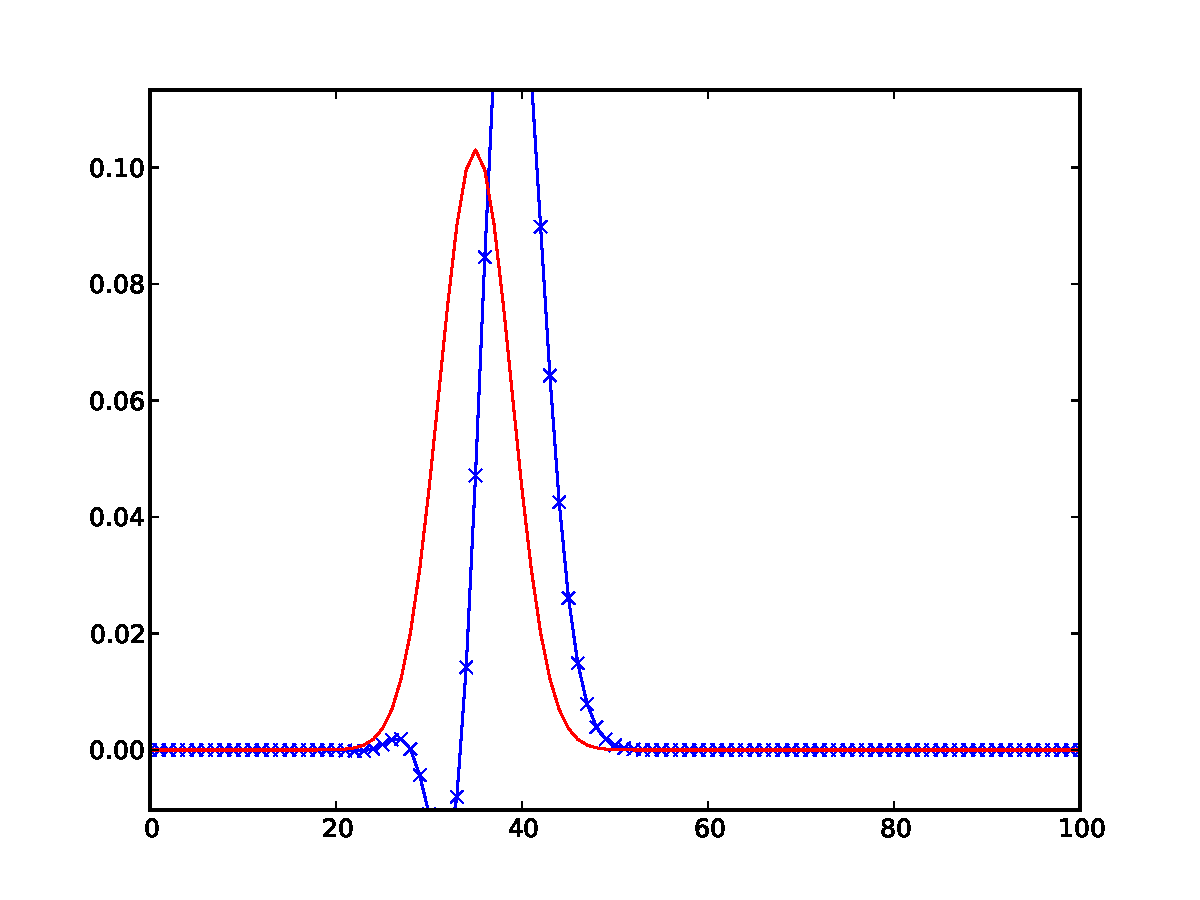
\includegraphics[width=0.5\textwidth]{ftcs10}
  \end{center}
  \label{fig:ftcs10}
\caption{The evolution of the Gaussian using FTCS after 10 time steps.}
\end{figure}

\begin{figure}[h]
  \begin{center}
     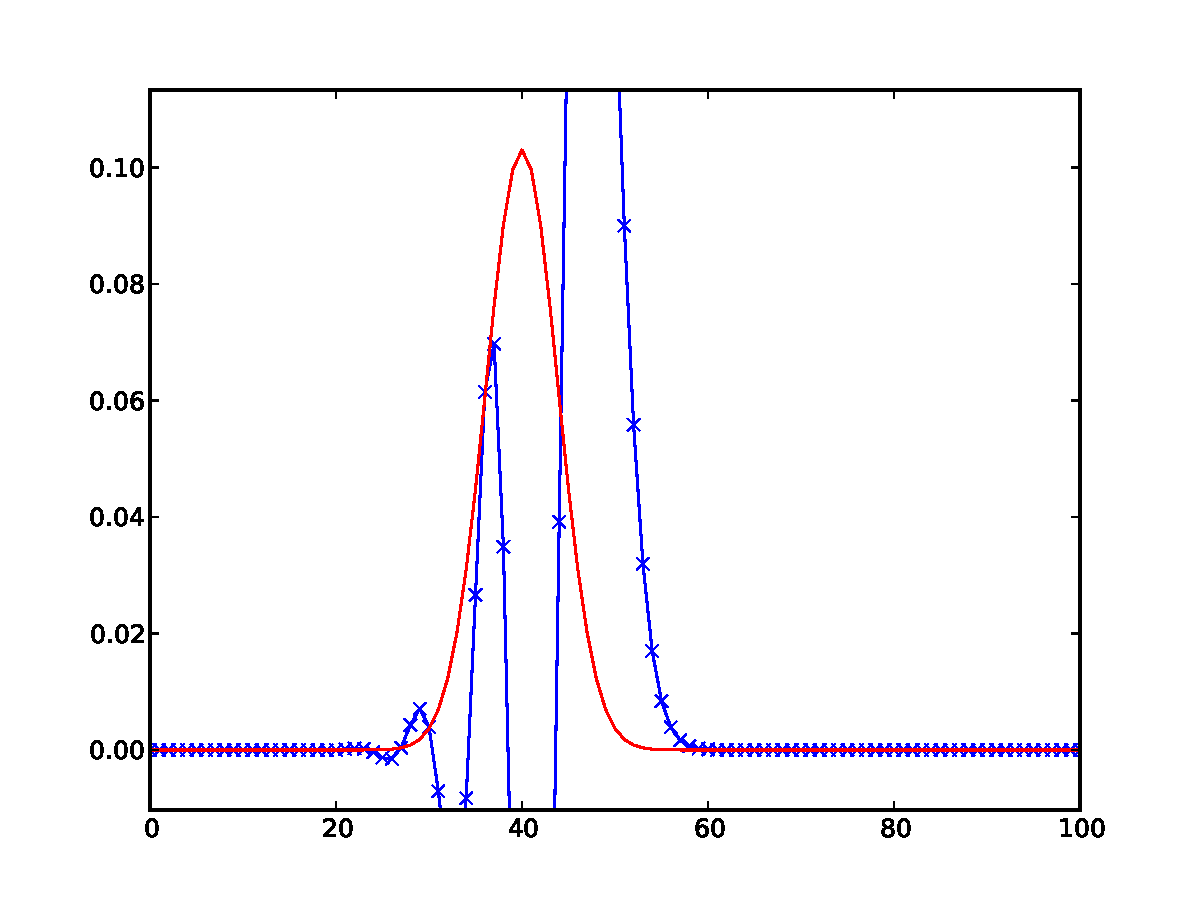
\includegraphics[width=0.5\textwidth]{ftcs20}
  \end{center}
  \label{fig:ftcs20}
\caption{The evolution of the Gaussian using FTCS after 20 time steps.}
\end{figure}

\section{Lax-Friedrich}
The Lax-Friedrich method is stable, but not quite as accurate as the upwind method.  Figure \ref{fig:compare}
compares the error over time for these two methods.

\begin{figure}[h]
  \begin{center}
     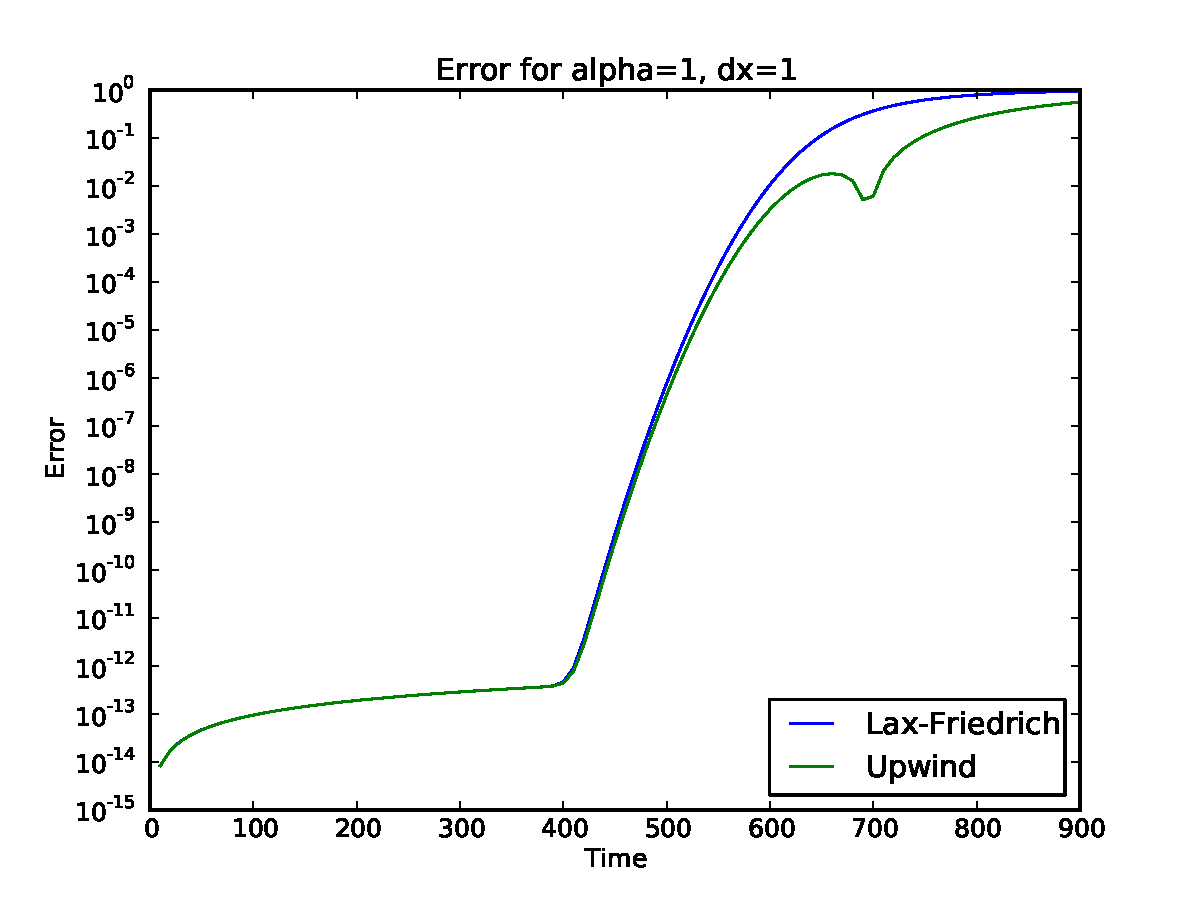
\includegraphics[width=\textwidth]{err_lf_vs_up}
  \end{center}
  \label{fig:compare}
\end{figure}

\section{Leapfrog and Lax-Wendroff}
The Lax-Wendroff method works fairly well.  The leapfrog method, on the other hand, may converge but it does not yield
pretty results along the way.  Oscillations appear in the leapfrog method, but then they die out, which I guess means that it
converges.  Figure \ref{fig:compare2} shows the error over time for these two methods.  Figure \ref{fig:con} shows the calculated
convergence rate for Lax-Wendroff at different points in time, calculated by comparing the error using dx=1 and the error using
dx=0.5.  The plot shows a convergence rate of 2 until the Gaussian starts to slide out of the field of view, at which point
things get complicated.

\begin{figure}[h]
  \begin{center}
     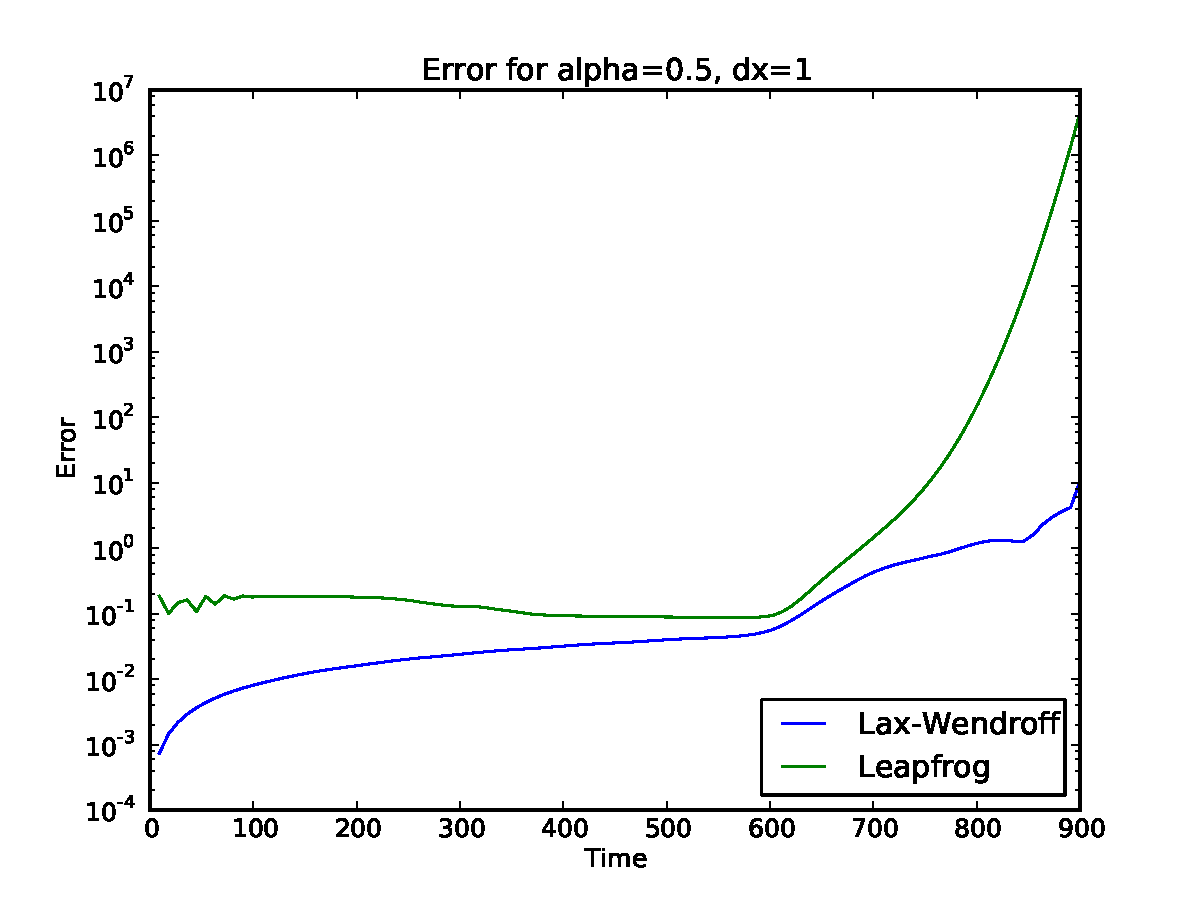
\includegraphics[width=\textwidth]{err_lw_vs_leap}
  \end{center}
  \label{fig:compare2}
\end{figure}

\begin{figure}[h]
  \begin{center}
     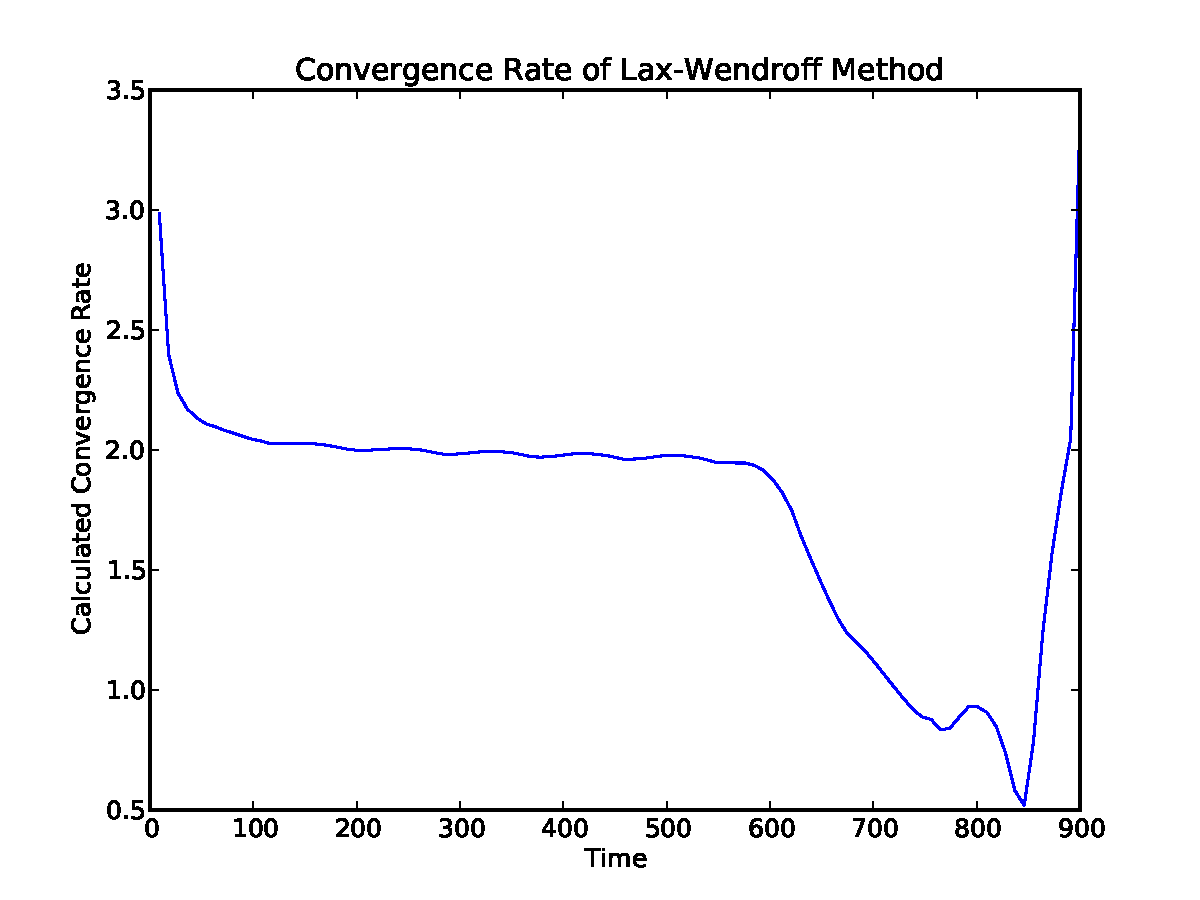
\includegraphics[width=\textwidth]{conv}
  \end{center}
  \label{fig:conv}
\end{figure}

\end{document}